\ifx\PREAMBLE\undefined
\documentclass{report}
\usepackage[format = hang, font = bf]{caption}
\usepackage{graphicx}
\usepackage{array}
\usepackage{amsmath}
\usepackage{mathtools}
\usepackage{boxedminipage}
\usepackage{listings}
\usepackage{makecell}%diagonal line in table
\usepackage{float}%allowing forceful figure[H]
\usepackage{xcolor}
\usepackage{amsfonts}%allowing \mathbb{R}
\usepackage{alltt}
\usepackage{algorithmicx}
\usepackage[chapter]{algorithm} 
%chapter option ensures that algorithms are numbered within each chapter rather than in the whole article
\usepackage[noend]{algpseudocode} %If end if, end procdeure, etc is expected to appear, remove the noend option
\usepackage{xspace}
\usepackage{color}
\usepackage{url}
\def\UrlBreaks{\do\A\do\B\do\C\do\D\do\E\do\F\do\G\do\H\do\I\do\J\do\K\do\L\do\M\do\N\do\O\do\P\do\Q\do\R\do\S\do\T\do\U\do\V\do\W\do\X\do\Y\do\Z\do\[\do\\\do\]\do\^\do\_\do\`\do\a\do\b\do\c\do\d\do\e\do\f\do\g\do\h\do\i\do\j\do\k\do\l\do\m\do\n\do\o\do\p\do\q\do\r\do\s\do\t\do\u\do\v\do\w\do\x\do\y\do\z\do\0\do\1\do\2\do\3\do\4\do\5\do\6\do\7\do\8\do\9\do\.\do\@\do\\\do\/\do\!\do\_\do\|\do\;\do\>\do\]\do\)\do\,\do\?\do\'\do+\do\=\do\#\do\-}
\usepackage[breaklinks = true]{hyperref}
\lstset{language = c++, breaklines = true, tabsize = 2, numbers = left, extendedchars = false, basicstyle = {\ttfamily \footnotesize}, keywordstyle=\color{blue!70}, commentstyle=\color{red!70}, frame=shadowbox, rulesepcolor=\color{red!20!green!20!blue!20}, numberstyle={\color[RGB]{0,192,192}}}
\mathchardef\myhyphen="2D
% switch-case environment definitions
\algblock{switch}{endswitch} 
\algblock{case}{endcase}
%\algrenewtext{endswitch}{\textbf{end switch}} %If end switch is expected to appear, uncomment this line.
\algtext*{endswitch} % Make end switch disappear
\algtext*{endcase}
\begin{document}
\fi
\chapter{Optimization}
\section{Intermediate code}
Intermediate code uses a language between the source language and the target language. It provides an intermediate level of abstraction: more details than the source and fewer details than the target. High-level source languages like \texttt{Cool} and \texttt{C} reveals less low-level conceptions such as registers, making it difficult to find room for optimization, while low-level languages like assembly language are often limited to a specific type of machine architecture. 

We will introduce the conception with an intermediate language that can be called a ``high level assembly language''. It uses register names, but has an unlimited number of registers. It uses control structures like assembly language. Opcodes are used, but some of them are higher level (e.g. \texttt{\color{red}push}, which will be translated into a few assembly instructions on a machine of a particular architecture). Each instruction is either binary ($\mathtt{\color{red}x\coloneqq y\:op\:z}$) or unary($\mathtt{\color{red}x\coloneqq op\:y}$). Arguments on the right are always registers or constants. This is actually a wide-used form of intermediate code called \textbf{three-address code}. In this language, every intermediate value will have its own name. 

Generating intermediate code is similar to generating assembly code, except that unlimited number of registers can be used, which renders easier code generation. If we use $\color{red}\mathtt{igen(e,t)}$ to denote the function that generates code for expression \texttt{e} and stores the result in register \texttt{t} , we will have 
\begin{align*}
\mathtt{igen}&\mathtt{(e_1 + e_2,t)=}\\
&\mathtt{igen(e_1,t_1)}\\
&\mathtt{igen(e_2,t_2)}\\
&\mathtt{t\coloneqq t_1 + t_2}
\end{align*}
\section{Optimization overview}
Optimizations can be performed at different times:
\begin{enumerate}
\item On AST
\begin{description}
\item[Pro]Machine independent
\item[Con]Too high level
\end{description}
\item On assembly language
\begin{description}
\item[Pro]Exposes the most optimization opportunities
\item[Con]Machine dependent. Has to be reimplemented when re-targeting to different architectures.
\end{description}
\item {\color{red}On intermediate language}
\begin{description}
\item[Pro]Machine independent. Exposes optimization opportunities.
\end{description}
\end{enumerate}
We will discuss optimizations performed on intermediate languages. The intermediate language we use can be described with the following CFG:
\begin{align*}
\mathtt{P\rightarrow\:}&\mathtt{SP\:|\:S}\\
\mathtt{S\rightarrow\:}&\mathtt{id\coloneqq id\:op\:id}\\
|\:&\mathtt{id\coloneqq op\:id}\\
|\:&\mathtt{push\:id}\\
|\:&\mathtt{id\coloneqq pop}\\
|\:&\mathtt{if\:id\:relop\:id\:goto\:L}\\
|\:&\mathtt{L:}\\
|\:&\mathtt{jump\:L}
\end{align*}
\texttt{Id}'s are registers, and can be substituted by constants when they serve as arguments. Typical operations are {\color{red}+,-,*,/}. 

A \textbf{basic block} is a maximal sequence of instructions with no labels (except for the first instruction) and no jumps(except for the last instruction). The execution can only jump into a basic block at the first instruction and jump out of it at the last instruction. There is no other way to jump into it, and all instructions inside the block are guaranteed to be executed sequentially before the execution jumps out. This property enables us to conduct a series of optimizations.

A \textbf{control flow graph} is a directed graph with basic blocks as nodes. An edge from block A to block B exists if the execution can pass from the last instruction in A to the first instruction in B. The body of a method can be represented as a control flow graph. There is one initial node, and all ``return'' nodes are terminals. 

The purpose of optimization is to \textbf{improve a program's resource utilization}. Most of the time we try to make the program run faster, i.e. reduce the execution time. Other resources that optimization could be concerned about are code size, memory footprint, network messages sent, disk accesses, power, etc. The bottom line is that optimization should not alter what the program computes.

For languages like \texttt{C} and \texttt{Cool} there are 3 granularities of optimizations:
\begin{description}
\item[Local optimization]Applies to an isolated basic block.
\item[Global optimization]Applies to an isolated control flow graph (method body).
\item[Inter-procedural optimization]Applies across method boundaries.
\end{description}
Local optimizations are performed by most mainstream compilers. Many of them also perform global optimizations. Few compilers touch inter-procedural optimizations, not only because it's hard to implement, but also because it often does not provide as much improvement as the first two. In practice, it is usually a wise decision not to implement the fanciest optimizations because they tend to be hard to implement, costly in compile time while not much payoff can be gained.
\section{Local optimization}
Local optimization focuses on a single basic block. There is no need to analyze the entire method body.
\subsection{Constant folding}
For an instruction $\mathtt{x\coloneqq y\:op\:z}$ in which \texttt{y,z} are both constants, $\mathtt{y\:op\:z}$ can be computed at compile time. E.g., $\mathtt{x\coloneqq 2 + 2\Rightarrow x\coloneqq 4}$.

Constants folding can be dangerous when the compiler and the target code it generates are run on different machines, which is not uncommon in reality, e.g. in most embedded platforms. The two machines might feature different round-offs of floating point numbers. If we do constant folding according to the floating point semantics of the compile machine directly at compile time, we may end up with unwanted result at runtime. An obvious solution is to keep full precision inside the compiler and represent floating pointer numbers as string literals, and leave it to the runtime machine to handle the round offs.
\subsection{Eliminate unreachable basic blocks}
By eliminating basic blocks that cannot be reached from the initial block, we can make the program smaller, and sometimes faster, because of cache effects.
\subsection{Common subexpression elimination}
Some optimizations can be simplified if each register occurs only once on the lhs of an assignment. Intermediate code can be rewritten into \textbf{single assignment form} by introducing new registers to substitute earlier appearances of registers that are assigned more than once. 

If a basic block is in single assignment form and a definition $\color{red}\mathtt{x\coloneqq}$ is the first use of \texttt{x} in a block, then when two assignments have the same rhs, they are guaranteed to compute the same value, which allows us saving the trouble of computing the same expression twice. We can simply substitute the second appearance of the rhs with the register assigned in its first appearance.
\subsection{Copy propagation}
if $\color{red}\mathtt{w\coloneqq x}$ appears in a block, subsequent use of \texttt{w} can be replaced with \texttt{x}.
\subsection{Dead instruction elimination}
if $\color{red}\mathtt{w\coloneqq rhs}$ appears in a basic block, and \texttt{w} does not appear anywhere else in the program, then the instruction is dead and can be eliminated.

Each local optimization does little by itself, but typically optimizations will interact with each other. Performing one optimization might enable another one. Thus the usual approach is to iterate until no more improvements can be made. The optimizer can also be stopped at any point to limit compilation time. 
\subsection{Peephole optimization}
Local optimizations can be applied directly to assembly code rather than to intermediate code. \textbf{Peephole optimization} is effective for improving assembly code. The ``peephole'' is a short sequence of contiguous instructions. The optimizer replaces the sequence with an equivalent but faster sequence. The process is repeated for maximum effect.
\section{Global optimization}
\subsection{Dataflow analysis}
In order to replace a use of \texttt{x} by a constant \texttt{k} we must make sure that on every path to the use of \texttt{x}, the last assignment to \texttt{x} is $\mathtt{x\coloneqq k}$. This condition is not trivial to check, considering the existence of loops and conditional branches. Global \textbf{dataflow analysis} is required to check this condition.

Global optimization tasks share several common traits:
\begin{itemize}
\item The optimization depends on knowing a property X at a particular point in program execution.
\item Proving X at any single point requires knowledge of the entire program.
\item It is OK to be conservative. If the optimization requires X being true, then we want to figure out whether X is definitely true or we don't know if X is true. It is always safe to say ``don't know''.
\end{itemize}
\subsection{Global constant propagation}
We use the following denotations to note the status of \texttt{x} at each program point:
\begin{description}
\item[$\bot$]: The statement never gets executed.
\item[C]: Constant C.
\item[$\top$]: \texttt{x} is not a constant.
\end{description}
Once we have the status of \texttt{x} at every program point, we can simply replace the use of \texttt{x} by the associated constant where the status of \texttt{x} is constant. In order to gain this information, we define a function $\mathtt{\color{red}C(x,s,in/out)}$ to compute information about the value of \texttt{x} before/after the statement \texttt{s}. In the following discussion, statement \texttt{s} has immediate predecessor statements $\mathtt{p_1,\dots,p_n}$. We have the following rules to infer the \texttt{in} status of one statement from the \texttt{out} of its predecessors.
\begin{enumerate}
\item If $\mathtt{C(p_i,x,out) = \top}$ for any \texttt{i}, then $\mathtt{C(s,x,in) = \top}$.
\item If $\mathtt{C(p_i,x,out) = c_i,\:C(p_j,x,out) = c_j,\:c_i\neq c_j}$, then $\mathtt{C(s,x,in) = \top}$.
\item If $\mathtt{C(p_i,x,out) = c}$ for at least one \texttt{i} and $\mathtt{C(p_i,x,out) = \bot}$ for all other \texttt{i}, then $\mathtt{C(s,x,in) = c}$.
\item If $\mathtt{C(p_i,x,out) = \bot}$ for all \texttt{i}, then $\mathtt{C(s,x,in) = \bot}$.  
\end{enumerate} 
Now we discuss the rules to infer the \texttt{out} status of a statement from its own \texttt{in} status.
\begin{enumerate}
\setcounter{enumi}{4}
\item If $\mathtt{C(s,x,in)=\bot}$, then $\mathtt{C(s,x,out)=\bot}$.
\item $\mathtt{C(x\coloneqq c,x,out)=c}$ if \texttt{c} is a constant.
\item $\mathtt{C(x\coloneqq f(\dots),x,out)=\top}$, if \texttt{f(\dots)} is not a constant.
\item If $\mathtt{y\neq x}$, then $\mathtt{C(y\coloneqq \dots,x,out)=C(y\coloneqq \dots,x,in)}$.
\end{enumerate}
We can gain information about status of \texttt{x} on all program points with the following algorithm:
\begin{enumerate}
\item For every entry \texttt{s} to the program, set $\mathtt{C(s,x,in)=\top}$.
\item Set $\mathtt{C(s,x,in/out)=\bot}$ everywhere else.
\item Repeat until the rules above are satisfied: pick statement \texttt{s} that does not satisfy the rules and update accordingly. 
\end{enumerate}

Special consideration needs to be taken when it comes to loops. If the \texttt{in} status of each statement relies on its predecessors, the reliance relation will form a cycle, making it impossible to obtain a result without assigning some initial values. The initial value $\bot$, which means ``by far the execution hasn't reached this point", is obviously a wise choice.

The rules above can actually be simplified by the idea of ordering among the 3 values : $\bot < \mathtt{C} < \top$. Note that different constants are not comparable to each other. Rules 1-4 can actually be written as 
\begin{equation*}
\mathtt{C(s,x,in)=\underset{i}{lub}(C(p_i,x,out))}
\end{equation*}
in which \texttt{lub} means least upper bound\footnote{We used this concept in the discussion of type checking}. The use of \texttt{lub} actually explains why the algorithm is guaranteed to terminate. All values start as $\bot$ and can only increase, thus the status at any point can change at most twice, which implies that the constant propagation algorithm is linear in program size: total number of steps $\leq$ 2 * Number of $\mathtt{C(\dots)}$ values to compute = 4 * Number of statements.
\subsection{Liveness analysis}
Once constants have been propagated, we would like to eliminate dead code. This involves the analysis of \textbf{liveness}. A variable \texttt{x} is live at statement \texttt{s} if 
\begin{itemize}
\item There exists a statement \texttt{s'} that uses \texttt{x}.
\item There is a path from \texttt{s} to \texttt{s'}.
\item That path has no intervening assignment to \texttt{x}.
\end{itemize}
A statement $\mathtt{x\coloneqq \dots}$ is dead code and can be removed if \texttt{x} is dead after the assignment. The propagation of liveness obeys the following rules:
\begin{enumerate}
\item $\mathtt{L(p,x,out) = \underset{i}{\cup}\:L(s_i,x,in)}$, in which $\mathtt{s_i}$ are successors of \texttt{p}.
\item $\mathtt{L(s,x,in)=true}$ if \texttt{s} refers to \texttt{x} on the rhs.
\item $\mathtt{L(x\coloneqq e,x,in)=false}$ if \texttt{e} does not refer to \texttt{x}.
\item $\mathtt{L(s,x,in)=L(s,x,out)}$ if \texttt{s} does not refer to \texttt{x}.
\end{enumerate}
We can obtain the liveness information of variables using the following algorithm, just as we did for constant propagation:
\begin{enumerate}
\item Initialize all $\mathtt{L(\dots)=false}$.
\item Repeat until all statements satisfy the rules above: pick \texttt{s} where the rules are not satisfied and update accordingly.
\end{enumerate}
A value can change from false to true but not the other way around, thus can change only once, which guarantees the termination of the algorithm.

Constant propagation is a forward analysis (information pushed from input to output), while liveness analysis is a backward analysis (information pushed from output to input). There exist other global dataflow analysis, and most of them can be classified as either forward or backward analysis. Most of them follow the methodology of \textbf{local rules relating information between adjacent program points}. 
\section{Register allocation}
Intermediate code uses unlimited temporaries, which simplifies code generation and optimization, but complicates final translation to assembly. The intermediate needs to be rewritten by assigning multiple temporaries to the same register without changing the behavior of the program, so that it uses no more temporaries than the number of machine registers. Register allocation is as old as compilers. 

The basic principle of register allocation is that \textbf{temporaries $t_1$ and $t_2$ can share the same register if at any point in the program at most one of them is live}. In other words, \textbf{if $t_1$ and $t_2$ are both live at any time of the program, they cannot share a register}.
\subsection{Register interference graph (RIG)}
\begin{figure}[ht]
\centering
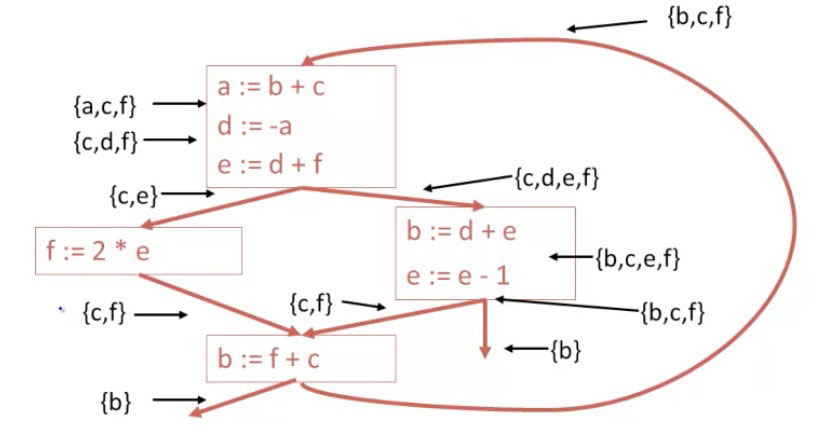
\includegraphics[width=0.7\textwidth]{liveness.jpg}
\caption{Liveness analysis of a program}\label{liveness}
\end{figure}

Take the program in Figure \ref{liveness} as an example. Its liveness analysis result is also shown. We can build an undirected graph according to this information. Each temporary is a node in the graph, and an edge is added between $t_1$ and $t_2$ if they are both live at some point in the program. The graph is called the \textbf{register interference graph (RIG)}. According to the principle above, two temporaries can share the same register as long as there is no edge between them in the RIG. The RIG of the program in Figure \ref{liveness} is shown in Figure \ref{rig}. In this example, \texttt{a} and \texttt{d} can use the same register since there is no edge between them.
\begin{figure}[ht]
\centering
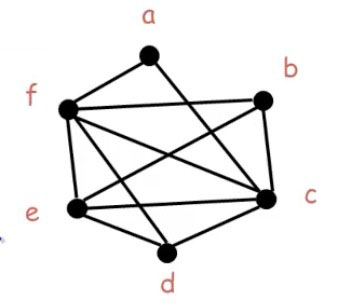
\includegraphics[width=0.3\textwidth]{rig.jpg}
\caption{RIG}\label{rig}
\end{figure}

RIG extracts exactly the information needed to carry out register allocation, and it provides a global (i.e. over the entire control flow graph) picture of the requirements for register allocation. After the construction of the RIG, the register allocation algorithm that we will present is architecture independent.
\subsection{Graph coloring}
A \textbf{coloring of graph} is an assignment of colors to nodes such that nodes connected by an edge have different colors. A graph is \textbf{k-colorable} if it can be colored using k or fewer colors. In our problem, if the RIG is k-colorable, then there must exist a register assignment that uses no more than k machine registers. The RIG shown in Figure \ref{rig} is 4-colorable.

We will take a divide-and-conquer approach to solve the problem.
\begin{itemize}
\item Pick a node \texttt{t} with \textbf{fewer} than \texttt{k} neighbors in the RIG.
\item Eliminate \texttt{t} and its edges from the RIG.
\item If the rest of the RIG is \texttt{k}-colorable, then so is the original RIG.
\end{itemize}
The logic is quite intuitive. Let $c_1,\dots,c_n(n<k)$ be the colors assigned to the neighbors of \texttt{t} in the reduced graph, then we can pick a color from the $k-n$ colors unused by these neighbors to color \texttt{t} in the original RIG. The whole process can be described as below.
\begin{enumerate}
\item Build the stack of nodes.
\begin{itemize}
\item Pick a node \texttt{t} with fewer than \texttt{k} neighbors.
\item Push \texttt{t} on the stack and remove it from the RIG.
\item Repeat until the RIG is empty.
\end{itemize}
\item Assign colors to nodes.
\begin{itemize}
\item Pop the node on top of the stack.
\item Color the node with a color different from those assigned to its neighbors, which have been popped out of the stack and colored in previous steps.
\end{itemize}
\end{enumerate}
\subsection{Spilling}
When the heuristic fails to find a coloring, it means that it is impossible to hold all temporaries in the registers. Some of them have to be \textbf{spilled} to the memory. 

When we get stuck in the heuristic, we will find that all nodes left in the RIG have k or more neighbors. We need to choose a node as a candidate for spilling. The associated value will have to live in the memory. The chosen node and its edges will then be removed from the RIG, and we continue the coloring with the rest of the RIG.
\ifx\PREAMBLE\undefined
\end{document}
\fi